\documentclass[border=3pt]{standalone}
% Preâmbulo compartilhado pelos diagramas TikZ da aula 8 de IHC (Design de IHC)
\usepackage[T1]{fontenc}
\usepackage[utf8]{inputenc}
\usepackage{lmodern}
\usepackage{amsmath}
\usepackage{xcolor}
\usepackage{tikz}
\usetikzlibrary{arrows.meta,angles,quotes,decorations.pathmorphing,decorations.pathreplacing,calc,
                positioning,shapes.geometric,shapes.misc,backgrounds,fit,
                math}

% Paleta (mesma dos SVGs originais)
% Paleta da disciplina de IHC: acento roxo (#755099), da capa do livro.
% (o nome "dblue" é mantido para não alterar todos os diagramas)
\definecolor{dblue}{HTML}{755099}
\definecolor{dorange}{HTML}{B3541E}
\definecolor{dgreen}{HTML}{4A7C59}
\definecolor{dred}{HTML}{9C4B4B}
\definecolor{dcream}{HTML}{F4F1EA}
\definecolor{dshade}{HTML}{DDD7C9}

% Função gaussiana (não normalizada por padrão de escala visual)
\pgfmathdeclarefunction{gauss}{3}{%
  \pgfmathparse{1/(#3*sqrt(2*pi))*exp(-((#1-#2)^2)/(2*#3^2))}%
}

% Estilos comuns (prefixo d... para não colidir com chaves internas do pgf)
\tikzset{
  >={Stealth[length=2mm]},
  dguide/.style={gray!55, dashed, line width=0.4pt},
  daxis/.style={gray!60, line width=0.7pt, ->},
  dbody/.style={fill=black!3, draw=black!80, line width=1pt},
  dacc/.style={draw=dblue, line width=1pt},
  dlbl/.style={black!55, font=\small},
  dsub/.style={black!45, font=\footnotesize},
  dstate/.style={circle, draw=black!80, fill=dcream, line width=1pt,
                 minimum size=17mm, font=\large, inner sep=1pt},
  dobs/.style={circle, draw=black!80, fill=dshade, line width=1pt,
               minimum size=14mm, font=\large, inner sep=1pt},
  dbox/.style={rounded corners=2pt, draw=black!80, fill=dcream, line width=1pt,
               align=center, inner sep=6pt},
  dop/.style={circle, draw=black!80, fill=white, line width=1pt,
              minimum size=6mm, inner sep=0pt, font=\small},
  dtrans/.style={->, dblue, line width=1pt},
  dmeas/.style={->, dorange, line width=1pt},
  dcurve/.style={line width=1pt, dblue},
  dcurveb/.style={line width=1.4pt, dorange},
}

\begin{document}
\hyphenpenalty=10000 \exhyphenpenalty=10000 \tolerance=9999 \emergencystretch=3em
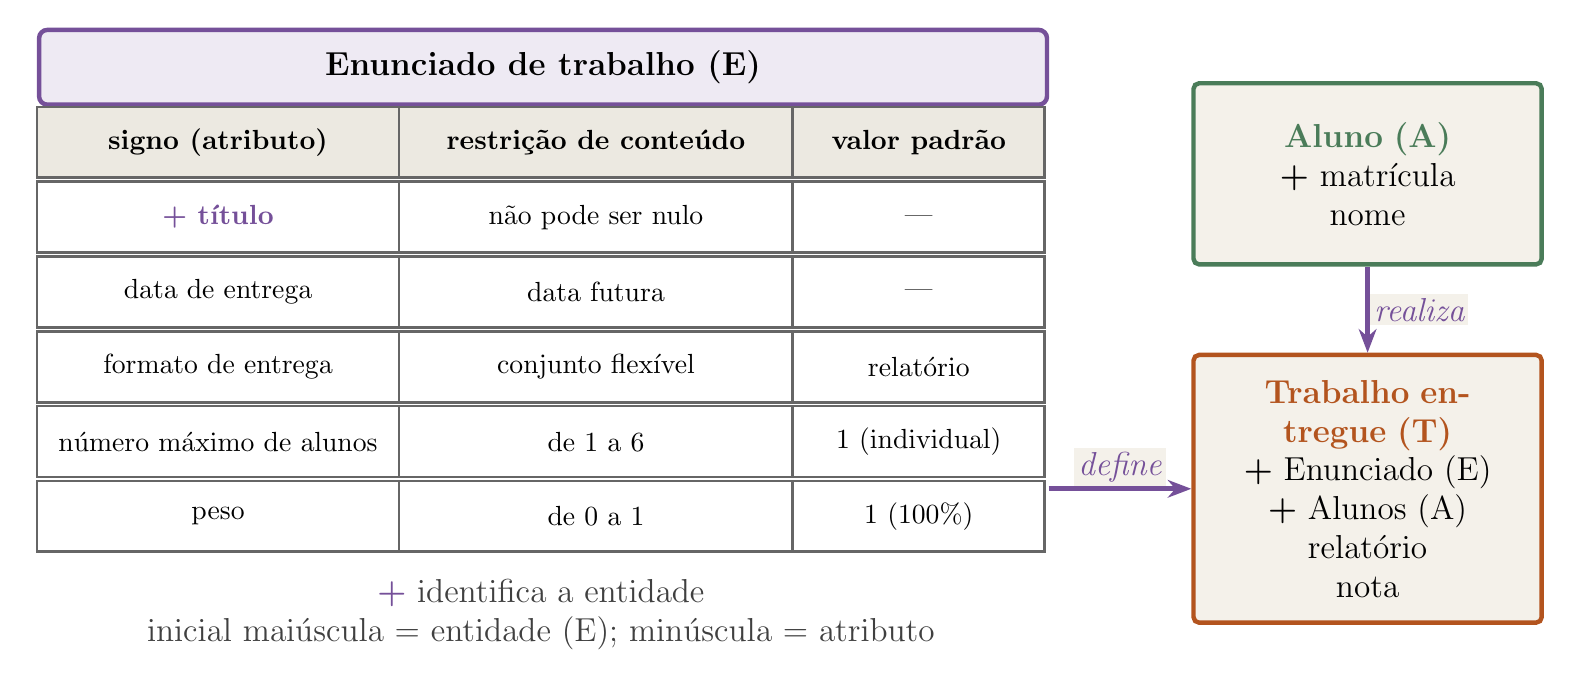
\begin{tikzpicture}[x=1cm,y=1cm]
\node[dbox, draw=dblue, fill=dblue!12, line width=1.6pt, minimum width=12.8cm, minimum height=0.95cm, font=\large\bfseries, anchor=south west, rounded corners=3pt] at (0,7.45) {Enunciado de trabalho (E)};
\draw[black!60, fill=dshade!55, line width=1pt] (0,6.55) rectangle (4.6,7.45);
\node[font=\normalsize\bfseries, text=black, text width=4.3cm, align=center] at (2.3,7.0) {signo (atributo)};
\draw[black!60, fill=dshade!55, line width=1pt] (4.6,6.55) rectangle (9.6,7.45);
\node[font=\normalsize\bfseries, text=black, text width=4.7cm, align=center] at (7.1,7.0) {restrição de conteúdo};
\draw[black!60, fill=dshade!55, line width=1pt] (9.6,6.55) rectangle (12.8,7.45);
\node[font=\normalsize\bfseries, text=black, text width=2.9cm, align=center] at (11.2,7.0) {valor padrão};
\draw[black!60, fill=white, line width=1pt] (0,5.6) rectangle (4.6,6.5);
\node[font=\normalsize\bfseries, text=dblue, text width=4.3cm, align=center] at (2.3,6.05) {+ título};
\draw[black!60, fill=white, line width=1pt] (4.6,5.6) rectangle (9.6,6.5);
\node[font=\normalsize, text=black, text width=4.7cm, align=center] at (7.1,6.05) {não pode ser nulo};
\draw[black!60, fill=white, line width=1pt] (9.6,5.6) rectangle (12.8,6.5);
\node[font=\normalsize, text=black, text width=2.9cm, align=center] at (11.2,6.05) {---};
\draw[black!60, fill=white, line width=1pt] (0,4.6499999999999995) rectangle (4.6,5.55);
\node[font=\normalsize, text=black, text width=4.3cm, align=center] at (2.3,5.1) {data de entrega};
\draw[black!60, fill=white, line width=1pt] (4.6,4.6499999999999995) rectangle (9.6,5.55);
\node[font=\normalsize, text=black, text width=4.7cm, align=center] at (7.1,5.1) {data futura};
\draw[black!60, fill=white, line width=1pt] (9.6,4.6499999999999995) rectangle (12.8,5.55);
\node[font=\normalsize, text=black, text width=2.9cm, align=center] at (11.2,5.1) {---};
\draw[black!60, fill=white, line width=1pt] (0,3.7) rectangle (4.6,4.6000000000000005);
\node[font=\normalsize, text=black, text width=4.3cm, align=center] at (2.3,4.15) {formato de entrega};
\draw[black!60, fill=white, line width=1pt] (4.6,3.7) rectangle (9.6,4.6000000000000005);
\node[font=\normalsize, text=black, text width=4.7cm, align=center] at (7.1,4.15) {conjunto flexível};
\draw[black!60, fill=white, line width=1pt] (9.6,3.7) rectangle (12.8,4.6000000000000005);
\node[font=\normalsize, text=black, text width=2.9cm, align=center] at (11.2,4.15) {relatório};
\draw[black!60, fill=white, line width=1pt] (0,2.75) rectangle (4.6,3.6500000000000004);
\node[font=\normalsize, text=black, text width=4.3cm, align=center] at (2.3,3.2) {número máximo de alunos};
\draw[black!60, fill=white, line width=1pt] (4.6,2.75) rectangle (9.6,3.6500000000000004);
\node[font=\normalsize, text=black, text width=4.7cm, align=center] at (7.1,3.2) {de 1 a 6};
\draw[black!60, fill=white, line width=1pt] (9.6,2.75) rectangle (12.8,3.6500000000000004);
\node[font=\normalsize, text=black, text width=2.9cm, align=center] at (11.2,3.2) {1 (individual)};
\draw[black!60, fill=white, line width=1pt] (0,1.8) rectangle (4.6,2.7);
\node[font=\normalsize, text=black, text width=4.3cm, align=center] at (2.3,2.25) {peso};
\draw[black!60, fill=white, line width=1pt] (4.6,1.8) rectangle (9.6,2.7);
\node[font=\normalsize, text=black, text width=4.7cm, align=center] at (7.1,2.25) {de 0 a 1};
\draw[black!60, fill=white, line width=1pt] (9.6,1.8) rectangle (12.8,2.7);
\node[font=\normalsize, text=black, text width=2.9cm, align=center] at (11.2,2.25) {1 (100\%)};
\node[font=\large, black!75, text width=12.8cm, align=center] at (6.4,1.0) {\textbf{\textcolor{dblue}{+}} identifica a entidade\\ inicial maiúscula = entidade (E); minúscula = atributo};
\node[dbox, draw=dgreen, line width=1.6pt, text width=4.0cm, minimum height=2.3cm, font=\large] (al) at (16.9,6.6) {\textbf{\textcolor{dgreen}{Aluno (A)}}\\ \textbf{+} matrícula\\ nome};
\node[dbox, draw=dorange, line width=1.6pt, text width=4.0cm, minimum height=3.4cm, font=\large] (tr) at (16.9,2.6) {\textbf{\textcolor{dorange}{Trabalho entregue (T)}}\\ \textbf{+} Enunciado (E)\\ \textbf{+} Alunos (A)\\ relatório\\ nota};
\draw[dtrans, line width=1.8pt, -{Stealth[length=3mm]}] (al.south) -- node[right, font=\large\itshape, fill=dcream, inner sep=1.5pt] {realiza} (tr.north);
\draw[dtrans, line width=1.8pt, -{Stealth[length=3mm]}] (12.85,2.6) -- node[above, font=\large\itshape, fill=dcream, inner sep=1.5pt] {define} (tr.west);
\end{tikzpicture}
\end{document}
